\chapter{Resultate}
\label{ch_resultat}

Im Kapitel \ref{ch_vorgehen} ist die Umsetzung ausführlich erklärt. In diesem Kapitel geht es um die relevanten Resultate. Diese teilen sich in die bekannten Kategorien Harvester, Energy - und Power Management sowie die BLE-Applikation. Die Resultate jeder Kategorie werden in einem Unterkapitel beschrieben.
 
\section{Harvesterschaltung}

\subsection{Der Print}

Das erste konkrete Resultat ist der fertige Print. In der Abbildung \ref{print_vorne} ist die Vorderseite abgebildet. \todo{bessere Beschreibung} Darauf befindet sich im Wesentlichen der Header als Verbindungsstecker zum Sensortag, die vier Gleichrichterdioden, der Limiter, die Spule und der EM8500. In der Abbildung \ref{print_rueckseite} befindet sich der Reed-Switch und die dreilagige Premo-Spule, mit der die Induktion erzeugt wird.

\begin{figure}[ht]
    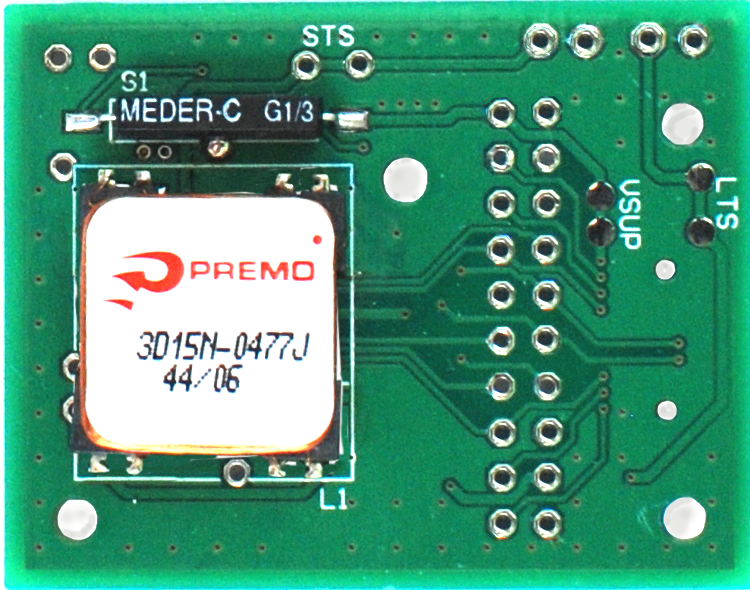
\includegraphics[width=0.5\textwidth]{4Resultate/imag/print_rueckseite.png} 
    \caption{Print Vorderseite}
    \label{print_vorne}
\end{figure}


\begin{figure}[ht]
    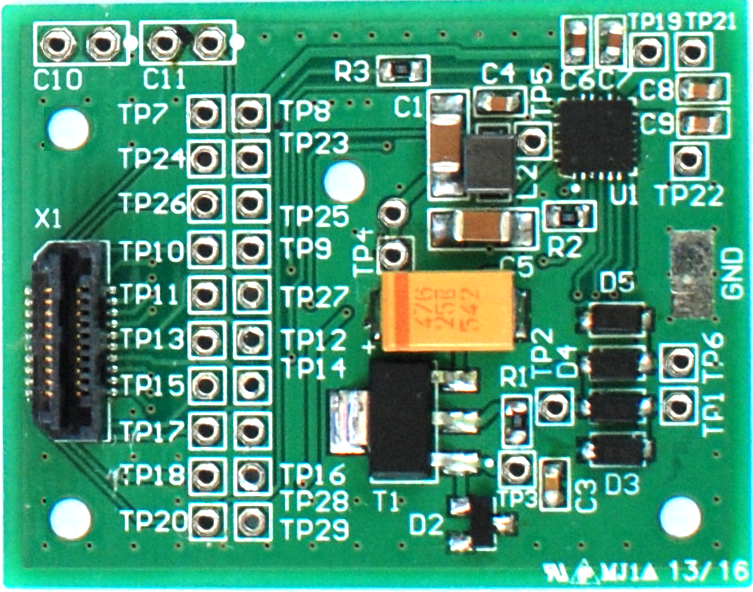
\includegraphics[width=0.5\textwidth]{4Resultate/imag/print_vorne.png} 
    \caption{Print Rückseite}
    \label{print_rueckseite}
\end{figure}

\newpage  % todel
\subsection{Leistung am Harvesterausgang}

Wie erwartet (siehe theoretische Grundlagen \ref{mpp_theorie_diff}) ändert sich bei einer Hardware mit Spule das Leistungsmaximum. Die Abbildung \ref{mpp_resultat_harvester} zeigt die reale MPP-Kurve des Prototypen. Bei 10 km/h liegt das Leistungsmaximum bei xxx mW, bei 15 km/h bei xxx mW, bei 20 km/h bei xxx mW und bei 40 km/h bei xxx mW. Die detaillierten Angaben finden sich im Messprotokoll xxxx \todo{Name Messprotokoll}.

\subsubsection*{Tabelle Leistung Harvesterausgang}
\begin{tabbing}
    Geschwindigkeit \quad\= Leistung Harvester \\[0.8ex]
    10 km/h  \> 21.87  $\mu$W \\
    15 km/h  \> 57.19  $\mu$W \\
    20 km/h> \> 114.67 $\mu$W \\
    40 km/h> \> 416.29 $\mu$W \\
\end{tabbing}  

\begin{figure}[ht]
    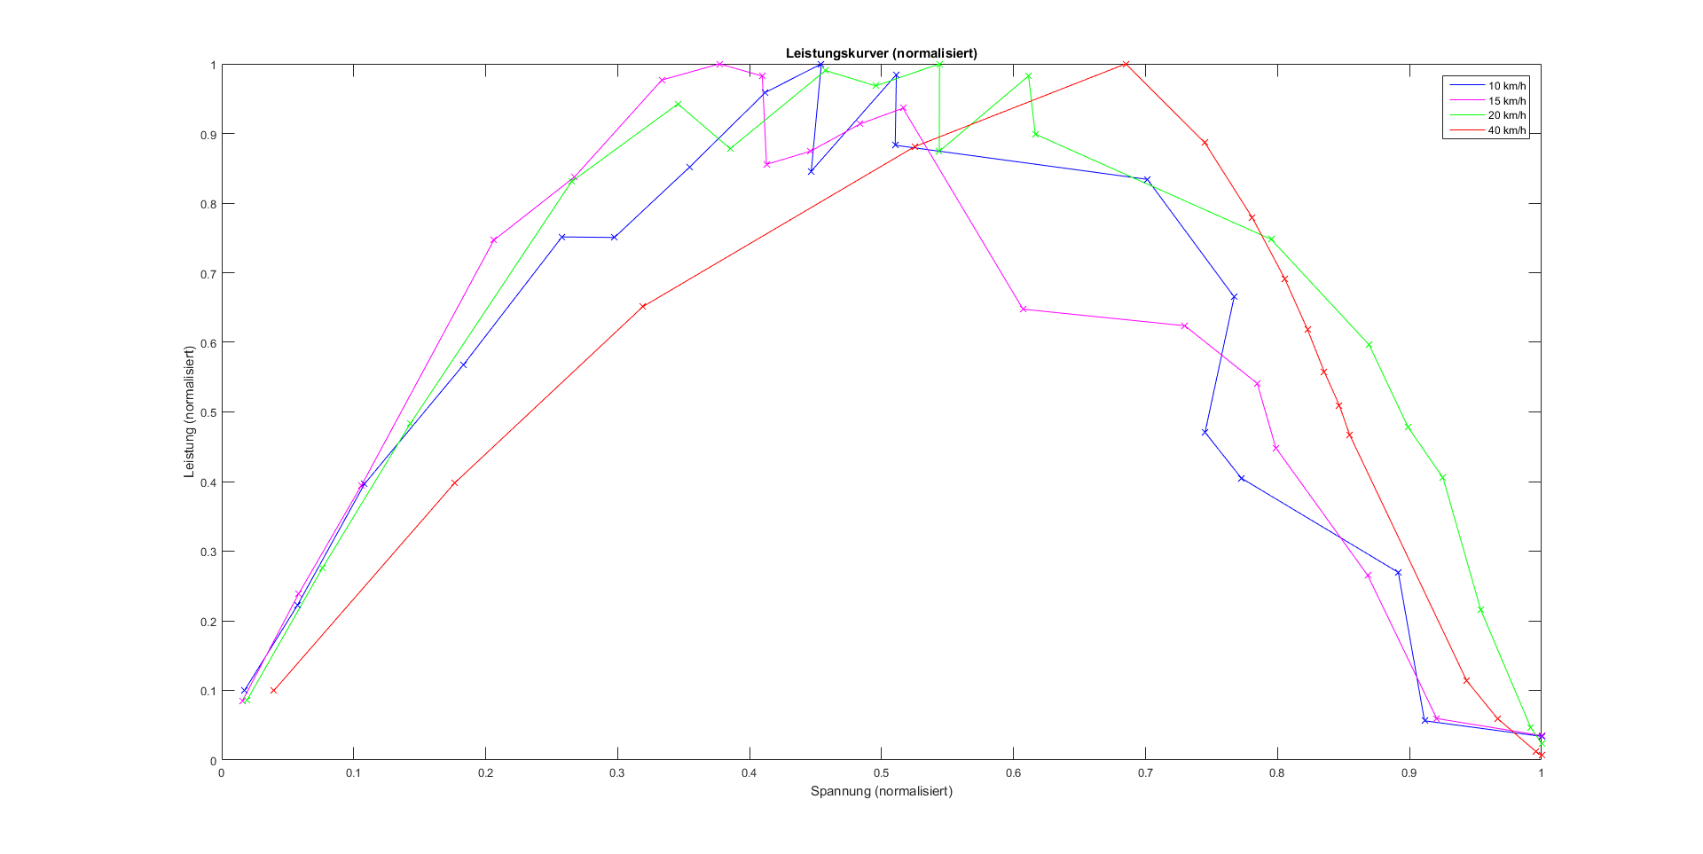
\includegraphics[width=0.5\textwidth]{4Resultate/imag/MPPHarvester.png} 
    \caption{Leistungskurve Harvesterausgang (normalisiert)}
    \label{mpp_resultat_harvester}
\end{figure}


\newpage  % todel
\subsection{Verhalten des Harvesterausgangs}

Die Abbildung \ref{resultat_Harvester_Spannung} zeigt, das reelle Verhalten des Harvesters bei Belastung mit dem EM-Chip. Wie in beschrieben \ref{optimaleLeistung} regelt der Chip EM8500 den Eingang, bzw. den Ausgang des Harvesters, um den MPP zu erreichen. Die Abbildung \ref{resultat_Harvester_Spannung} zeigt den Verlauf der geregelten Spannung am Eingang des EM-Chips über längere Zeit. Weitere Messungen zum reelen Verhalten am EM8500-Chip-Eingang können den Messprotokoll \todo{Namen heraussuchen} entnommen werden.


\begin{figure}[ht]
    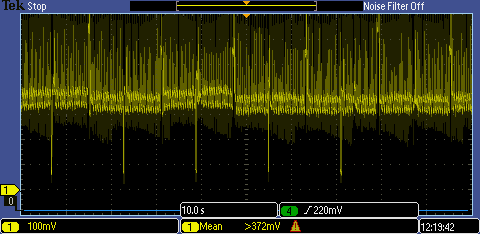
\includegraphics[width=0.5\textwidth]{4Resultate/imag/SpannungVCC.png} 
    \caption{Spannung VCC beim Harvesterausgang bei 15 km/h}
    \label{resultat_Harvester_Spannung}
\end{figure}

\newpage  % todel
\subsection{Energie am EM-Chipausgang}

Die Abbildung \ref{energie_resultat_harvester} zeigt die berechnete Energie, die am Ausgang des EM-Chip abgegeben wird in Bezug zur Geschwindigkeit. Die Berechnung, wie aus dem Puls über die Zeit, bis dass VSUP wieder eingeschalten wird, ist im  Messprotokoll yyy dokumentiert. Die gewonnene Energie, die dem Sensortag zur Verfügung steht ist:

\subsubsection*{Tabelle Leistung und Wirkungsgrad }
\begin{tabbing}
    Geschwindigkeit \quad\= Leistung EM8500\_out \\[0.8ex]
    10 km/h  \> 5.44   $\mu$W\\
    15 km/h  \> 20.91  $\mu$W\\
    20 km/h> \> 41.39  $\mu$W\\
    40 km/h> \> 170.75 $\mu$W\\
\end{tabbing}  


\begin{figure}[ht]
    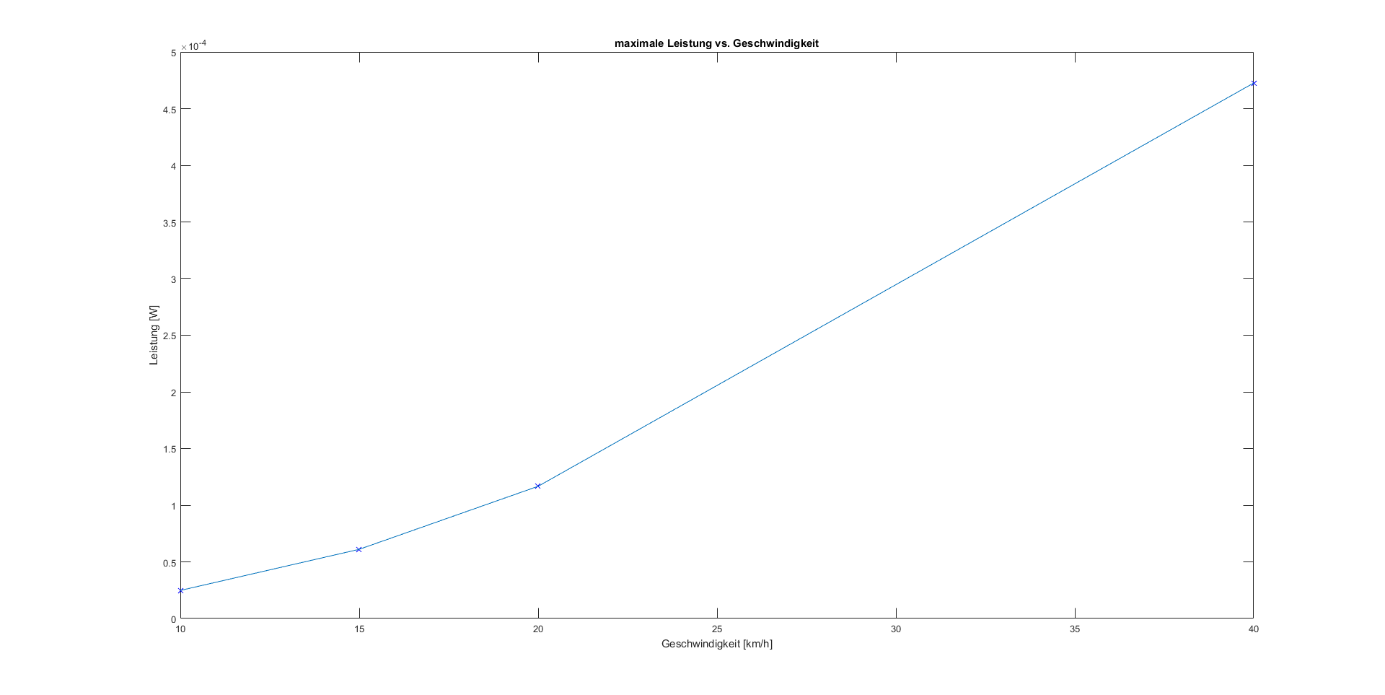
\includegraphics[width=0.5\textwidth]{4Resultate/imag/ResultatLeistungGeschwindigkeit.png} 
    \caption{Maximale Leistung vs. Geschwindigkeit}
    \label{energie_resultat_harvester}
\end{figure}

\subsection{Wirkungsgrad des Prototypen}

Aus den zwei Leistungsmessungen wird graphisch die Energiegewinnung im Vergleich dargestellt (Abbildung \ref{zsmEnergyGewinn}). Die Werte beziehen sich auf die gemittelte Leistung über 10 s. Es ist u sehen, dass die Energiegewinnung bei der Harvesterschaltung mit der Geschwindigkeit deutlich schneller zunimmt, als die Energie am Ausgang des EM-Chips. 

\begin{figure}[ht]
    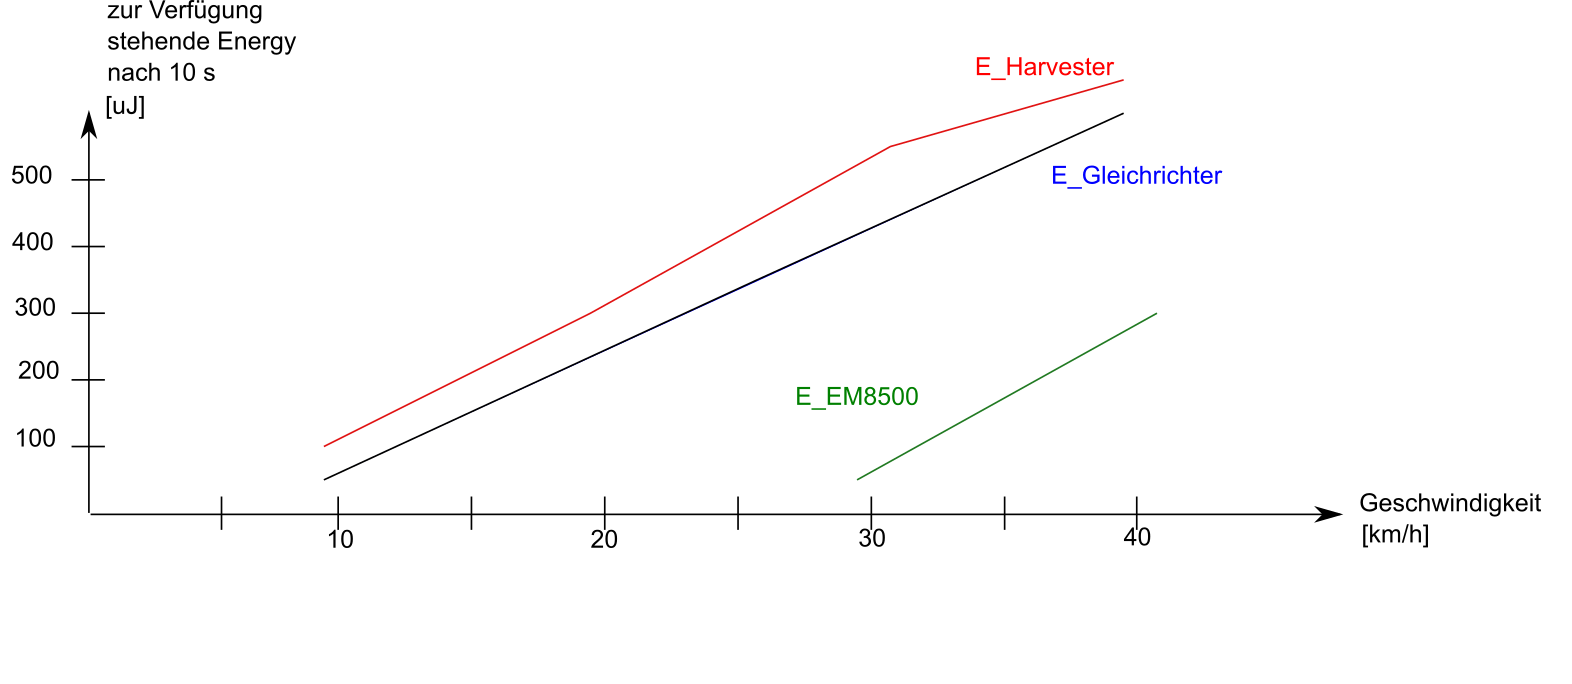
\includegraphics[width=1\textwidth]{4Resultate/imag/EnergyGewinnNachStelle.png} 
    \caption{Energiegewinn Zusammengefasst nach Stelle in der Schaltung}
    \label{zsmEnergyGewinn}
\end{figure}

Aus den zwei Leistungsmessungen wurde der Wirkungsgrad bei den gemessenen Geschwindigkeiten berechnet (siehe Tabelle unten). Der Wirkungsgrad ist bei tiefen Geschwindigkeiten sehr schlecht (24.87\thinspace\%). Dies ist eine der zwei Ursache, dass trotz genug geernteter Energie, das Sensortag für das Senden der Sensorwerte bei tiefer Geschwindigkeiten nicht wie erwartet genug Energie hat. Mit mehr Geschwindigkeit, erhöht sich nicht nur die geerntete Leistung rapide, sondern auch der Wirkungsgrad. Der Wirkungsgrad des EM8500 innerhalb des entwickelten Prototypen liegt bei 40 km/h  bei 41.01\thinspace\%.  

\subsubsection*{Tabelle Leistung und Wirkungsgrad }
\begin{tabbing}
    Geschwindigkeit \quad\= Leistung Harvester \quad\= Leistung EM8500\_out \quad\= Wirkungsgrad\\[0.8ex]
    10 km/h  \> 21.87  $\mu$W \> 5.44   $\mu$W \> 24.87\thinspace\%  \\
    15 km/h  \> 57.19  $\mu$W \> 20.91  $\mu$W \> 36.56\thinspace\%  \\
    20 km/h \> 114.67 $\mu$W \> 41.39  $\mu$W \> 36.09\thinspace\%  \\
    40 km/h \> 416.29 $\mu$W \> 170.75 $\mu$W \> 41.01\thinspace\%  \\
\end{tabbing}   



\section{Energy Management}

%Beim Resultat spielt das Hard- und Softwaremanagment direkt ineinander, weshalb das Ergebnisse dieser zwei Aufgaben zusammen dargestellt werden.

Das Ziel beim Energy Management ist, dass die vom Long Time Storage gespeicherte Energie für das Versenden der BLE-Pakete genutzt wird. Dies ist (siehe Abbildung \ref{LTSladet}) möglich. Die gesammelte Energie beider Kondensatoren wird für das Sender der BLE-Pakete verwendet. Die benutzten Kondensatorenwerte sind:

STS = 100 $\mu$F

LTS = 2200 $\mu$F

Die Werte ergaben sich aus folgender Energiekalkulation
\begin{equation}
W=\frac{1}{2}\cdot 100 uF \cdot (3.6 - 2.2 V)^{2}=xxxxx uW\label{eq:Energie STS}
\end{equation}

\begin{equation}
W=\frac{1}{2}\cdot 2.2 mF \cdot (3.6 - 2.2 V)^{2}=xxxxx mW\label{eq:Energie LTS}
\end{equation}


Dadurch sammelt STS in einer Periode von xx ms eine Enegrigemenge von \todo{finale Zeiten eintragen. Energie dafür eintragen} yyy mJ. LTS lädt in der Periode von  zz ms zusätzlich eine Energiemenge von yyy mJ. Die angereicherte Menge von tt mJ genügen, um ein xxx-Paket zu versenden.

\todo{besseres Bild}

\begin{figure}[ht]
    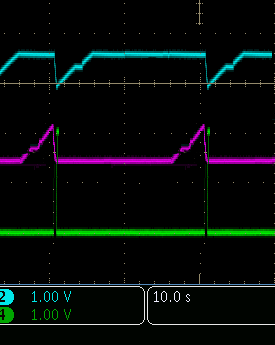
\includegraphics[width=0.5\textwidth]{4Resultate/imag/FakeLTSEntaden.png} 
    \caption{LTS liefert Energie für die Arbeitspakete}
    \label{LTSladet}
\end{figure}

Gelungen ist das Laden und Entladen beider Kondensatoren durch folgende EM-Schwellwerte:

\todo{correct space in table}
% Values from V1
\subsubsection*{Tabelle Finale Konfiguration Schwellwerte }
\begin{tabbing}
    Register .............\quad\= Spannungswert \\[0.8ex]
    v\_bat\_max\_hi       \> 3.9 V \\
    v\_bat\_max\_lo       \> 3.8 V \\
    v\_bat\_min\_hi\_dis  \> 3.6 V \\
    v\_bat\_min\_hi\_con  \> 2.2 V \\
    v\_bat\_min\_lo       \> 2.0 V \\
    v\_appl\_max\_hi      \> 3.8 V \\
    v\_appl\_max\_lo      \> 3.7 V \\   
\end{tabbing}  



\section{Powermanagement}

Lange schien es so, dass die Sensoren, aufgrund des grossen Verbrauchs der I2C-Kommunikation und der langen Aufstartzeit der Sensoren, nicht per BLE bei tiefer Geschwindigkeit gesendet werden können. Eine Lösung wurde möglich, weil Aufgabenblöcke in Unterblöcke mit Schlafensezeiten eingebaut wurden. Die untenstehende Tabelle zeit die gefunden Lösung:

\subsubsection*{Tabelle Energieverbrauch Aufgabenblöcke}
\begin{tabbing}
    Funktion ...................................................................................\quad\= Energieverbrauch \\[0.8ex]
    Auslesen Reed Switch und Berechnen Geschwindigkeit       \> xx mW \\
    Starten und Auslesen Drucksensor          \> xx mW \\
    Starten und Auslesen Temperatursensor     \> xx mW \\
    Starten und Auslesen Feuchtigkeitssensor  \> xx mW \\
    Auslesen Statusregister per SPI           \> xx mW \\
\end{tabbing}  


Die Lösung ist das Aufsplitten von Aufgabenblöcken. Bei genug Energie, wird nicht ein Sensor gestartet, ausgelesen und seine Daten versendet, sondern der Sensor wird gestartet, dann geht das System schlafen, bis dass LTS voll ist. Dann folgt der nächste Aufgabe: die Werte auslesen. Es wird wieder geschlafen und beim dritten Mal genügend Energie wird das Paket versendet. Das Konzept des Schlaffens zwischen Aufgabeblöcken ist im theoretischen Teil im Unterkapitel \ref{pm_sleep} im Abschnitt \ref{schlafen_theorie} beschrieben . Die Abbildung \ref{arbeitsaufteilung} zeigt, das Aufteilen der Arbeitsschritte: Zuerst folgt die Initialisierung des Sensors, dann folgt das Auslesen der Daten und zum Schluss das Senden der Werte.

\todo{Bild Arbeitsaufteilung }
\begin{figure}[ht]
    
\includegraphics[width=0.4\textwidth]{idle.png}
    %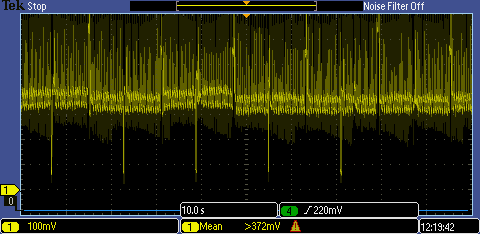
\includegraphics[width=0.1\textwidth]{4Resultate/imag/SpannungVCC.png} 
    \caption{Aufteilen in drei Schritte bis zum Senden der Daten}
    \label{arbeitsaufteilung}
\end{figure}

% ev. Grossaufnahme: BLE Energieverbrauch

Das Ergebnis ist in der Abbildung \ref{Sensor_Energie} graphisch dargestellt. Es zeigt sich, dass das Senden von Sensordaten \todo{Wert eintragen Tabelle und Text} xx mal mehr Energie verbrauchen, als das Senden der Geschwindigkeit. Die schlechteste Bilanz hat das Auslesen des Status Registers aus dem EM8500-Chip. In diesem Byte ist hinterlegt, welche Schwellwerte des EM8500 überschritten wurden und dient dadurch auf einfache Art dem Abbilden des aktuellen Energiezustands (siehe Unterkapitel \ref{v_energiezustand}). 

\begin{figure}[ht]
    
\includegraphics[width=0.4\textwidth]{idle.png}
    %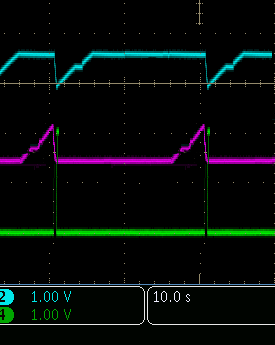
\includegraphics[width=0.5\textwidth]{4Resultate/imag/FakeLTSEntaden.png} 
    \caption{LTS liefert Energie für die Arbeitspakete}
    \label{Sensor_Energie}
\end{figure}


Kombiniert man den Energieverbrauch mit der zur Verfügung stehenden Energie am Ausgang nach dem EM8500-Chips, können (siehe Abbildung \ref{resultat_Zsm_Energy}) folgende Schlussfolgerungen gezogen werden:

\todo{ genauere Angaben nach Endmessungen}
\begin{enumerate}
    \item Das Übermitteln der Geschwindigkeit ist ab 10 km/h möglich
    \item Das Übermitteln aller Sensordaten (gestaffelt) ist ab xxx km/h möglich
    \item Das Übermitteln aller Sensordaten braucht bei einer Geschwindigkeit von 10 km/h xxxx s
    \item Das Übermitteln aller Sensordaten braucht bei 40 km/h xxx s
\end{enumerate}

\begin{figure}[ht]
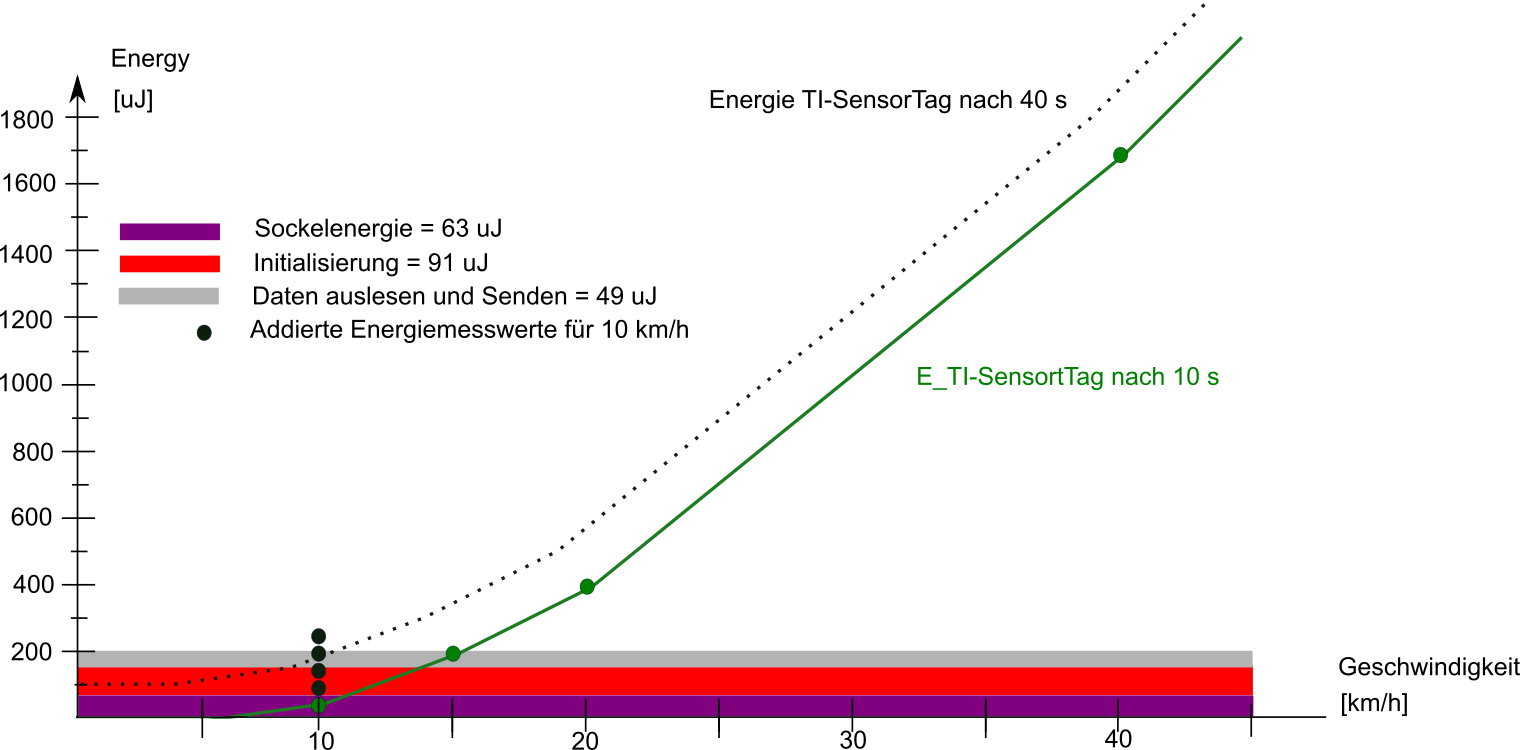
\includegraphics[width=1\textwidth]{4Resultate/imag/EnergyVerbrauchZusammenfassung.png}\label{resultat_Zsm_Energy} 
\caption{Energieverbrauch gem\"{a}ss Verarbeitungsaufwand für CPU}
\end{figure}






\newpage
\section{Ergebnisse BLE-Applikation}

Der Aufbau des Sensortags zusammen mit dem selbst entwickelten Board wird \glqq Sensor\grqq\thinspace\ genannt. Dies, weil aus der Sicht einer Benutzerin oder eines Benutzers keine detaillierte Hardware besteht, sondern \glqq ein Sensor\grqq. Die Vereinfachung dient der Benutzerfreundlichkeit. Die Android-Applikation ist bewusst einfach aufgebaut, um die Benutzerin bzw. den Benutzer nicht zu verwirren. 

Der animierte Tachometer stellt die aktuelle Geschwindigkeit schnell und übersichtlich dar. Weitergehende Funktionen sind durch prägnante Namen selbsterklärend und der User sollte keine Mühe haben, die App ohne Lesen einer Anleitung zu verstehen.

\subsection{Applikationsstruktur}

Beim Öffnen der Applikation wird geprüft, ob Bluetooth aktiviert ist (siehe Abbildung \ref{permission}). Sollte Bluetooth nicht aktiviert sein, wird der User gefragt, ob Bluetooth aktiviert werden darf. Sollte der User die Aktivierung ablehnen schliesst sich die Applikation sofort.

\begin{figure}[ht]
    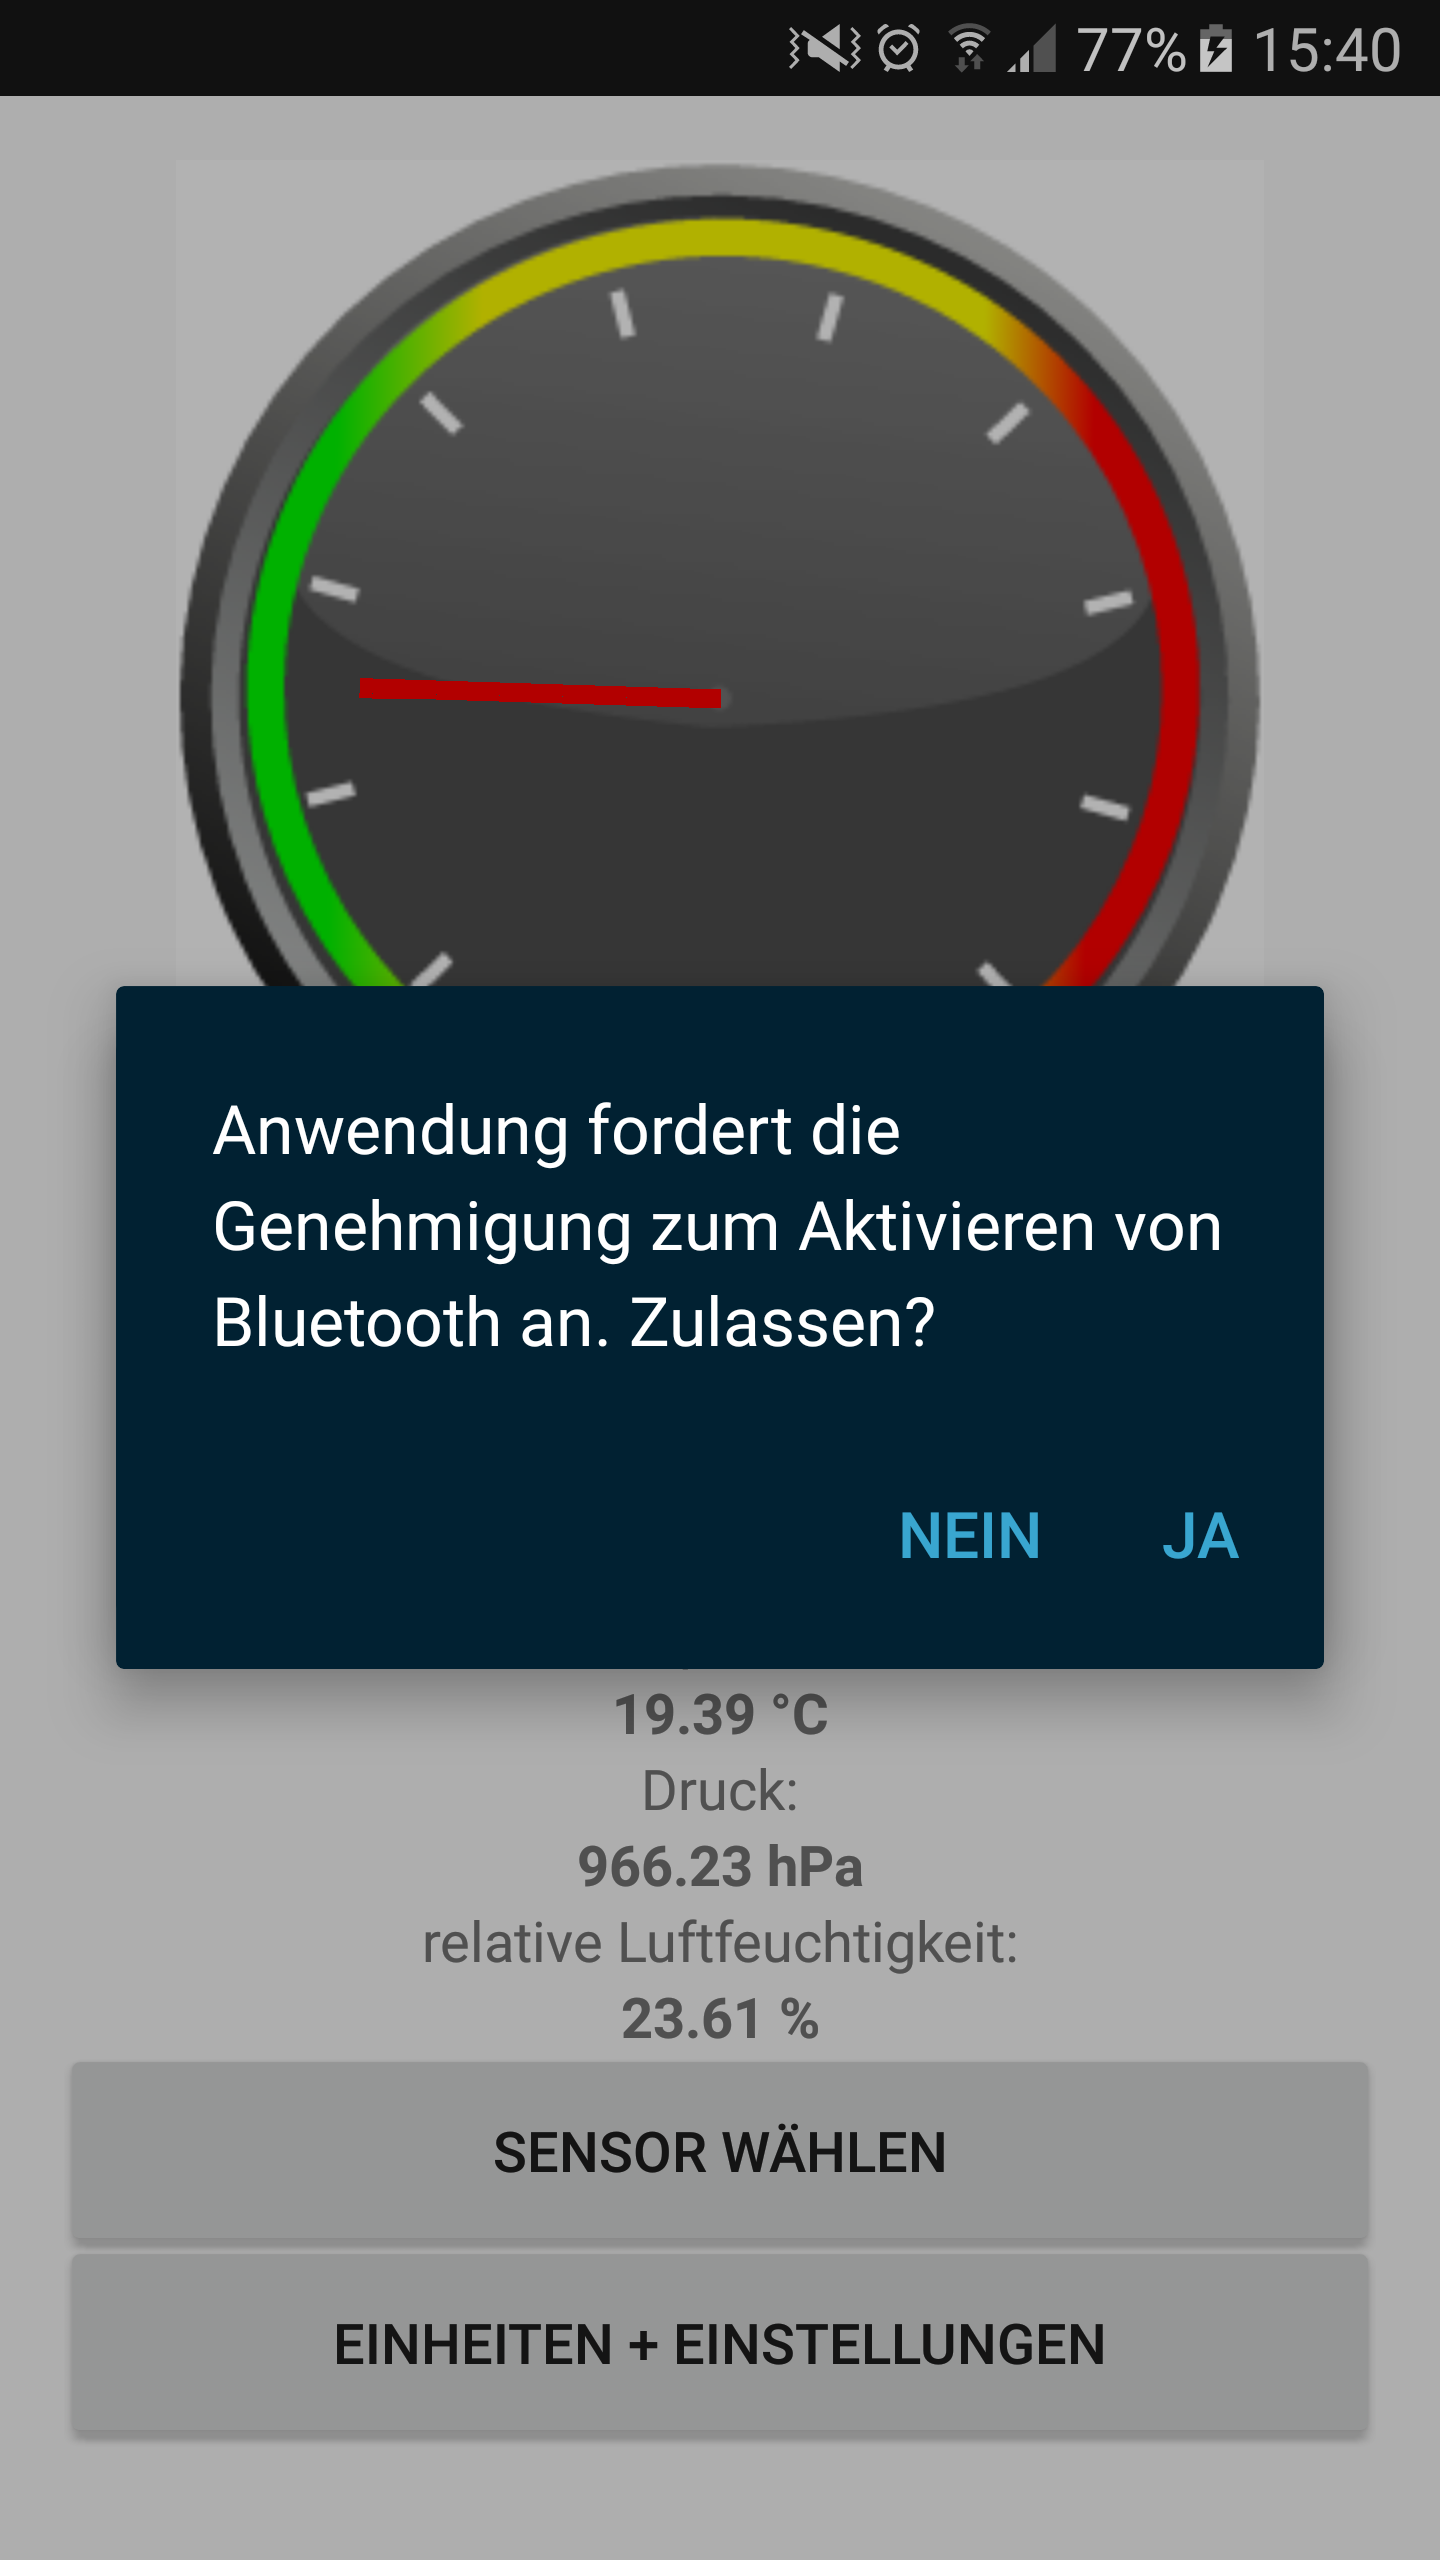
\includegraphics[width=0.5\textwidth]{4Resultate/imag/BLEBluetoothPermission.png} 
    \caption{Bluetooth Permission}
    \label{permission}
\end{figure}

Wird eine Verbund zu Bluetooth erlaubt, erscheint der Startbildschirm. Auf diesem befindet sich zentral der Tachometer (siehe Abbildung \ref{tacho}). Dieser zeigt Geschwindigkeiten von 0 – 90 km/h mit einer animierten Tachonadel an. Unterhalb des Tachometers werden die einzelnen Sensordaten angezeigt und im untersten Teil des Startbildschirms befinden sich zwei Buttons, über die man Einstellungen vornehmen kann. Die Kontextmenus zu diesen Einstellungen werden in den nächsten zwei Abbildungen \ref{sensorauswahl} und \ref{einheiten} ersichtlich. 

\begin{figure}[ht]
    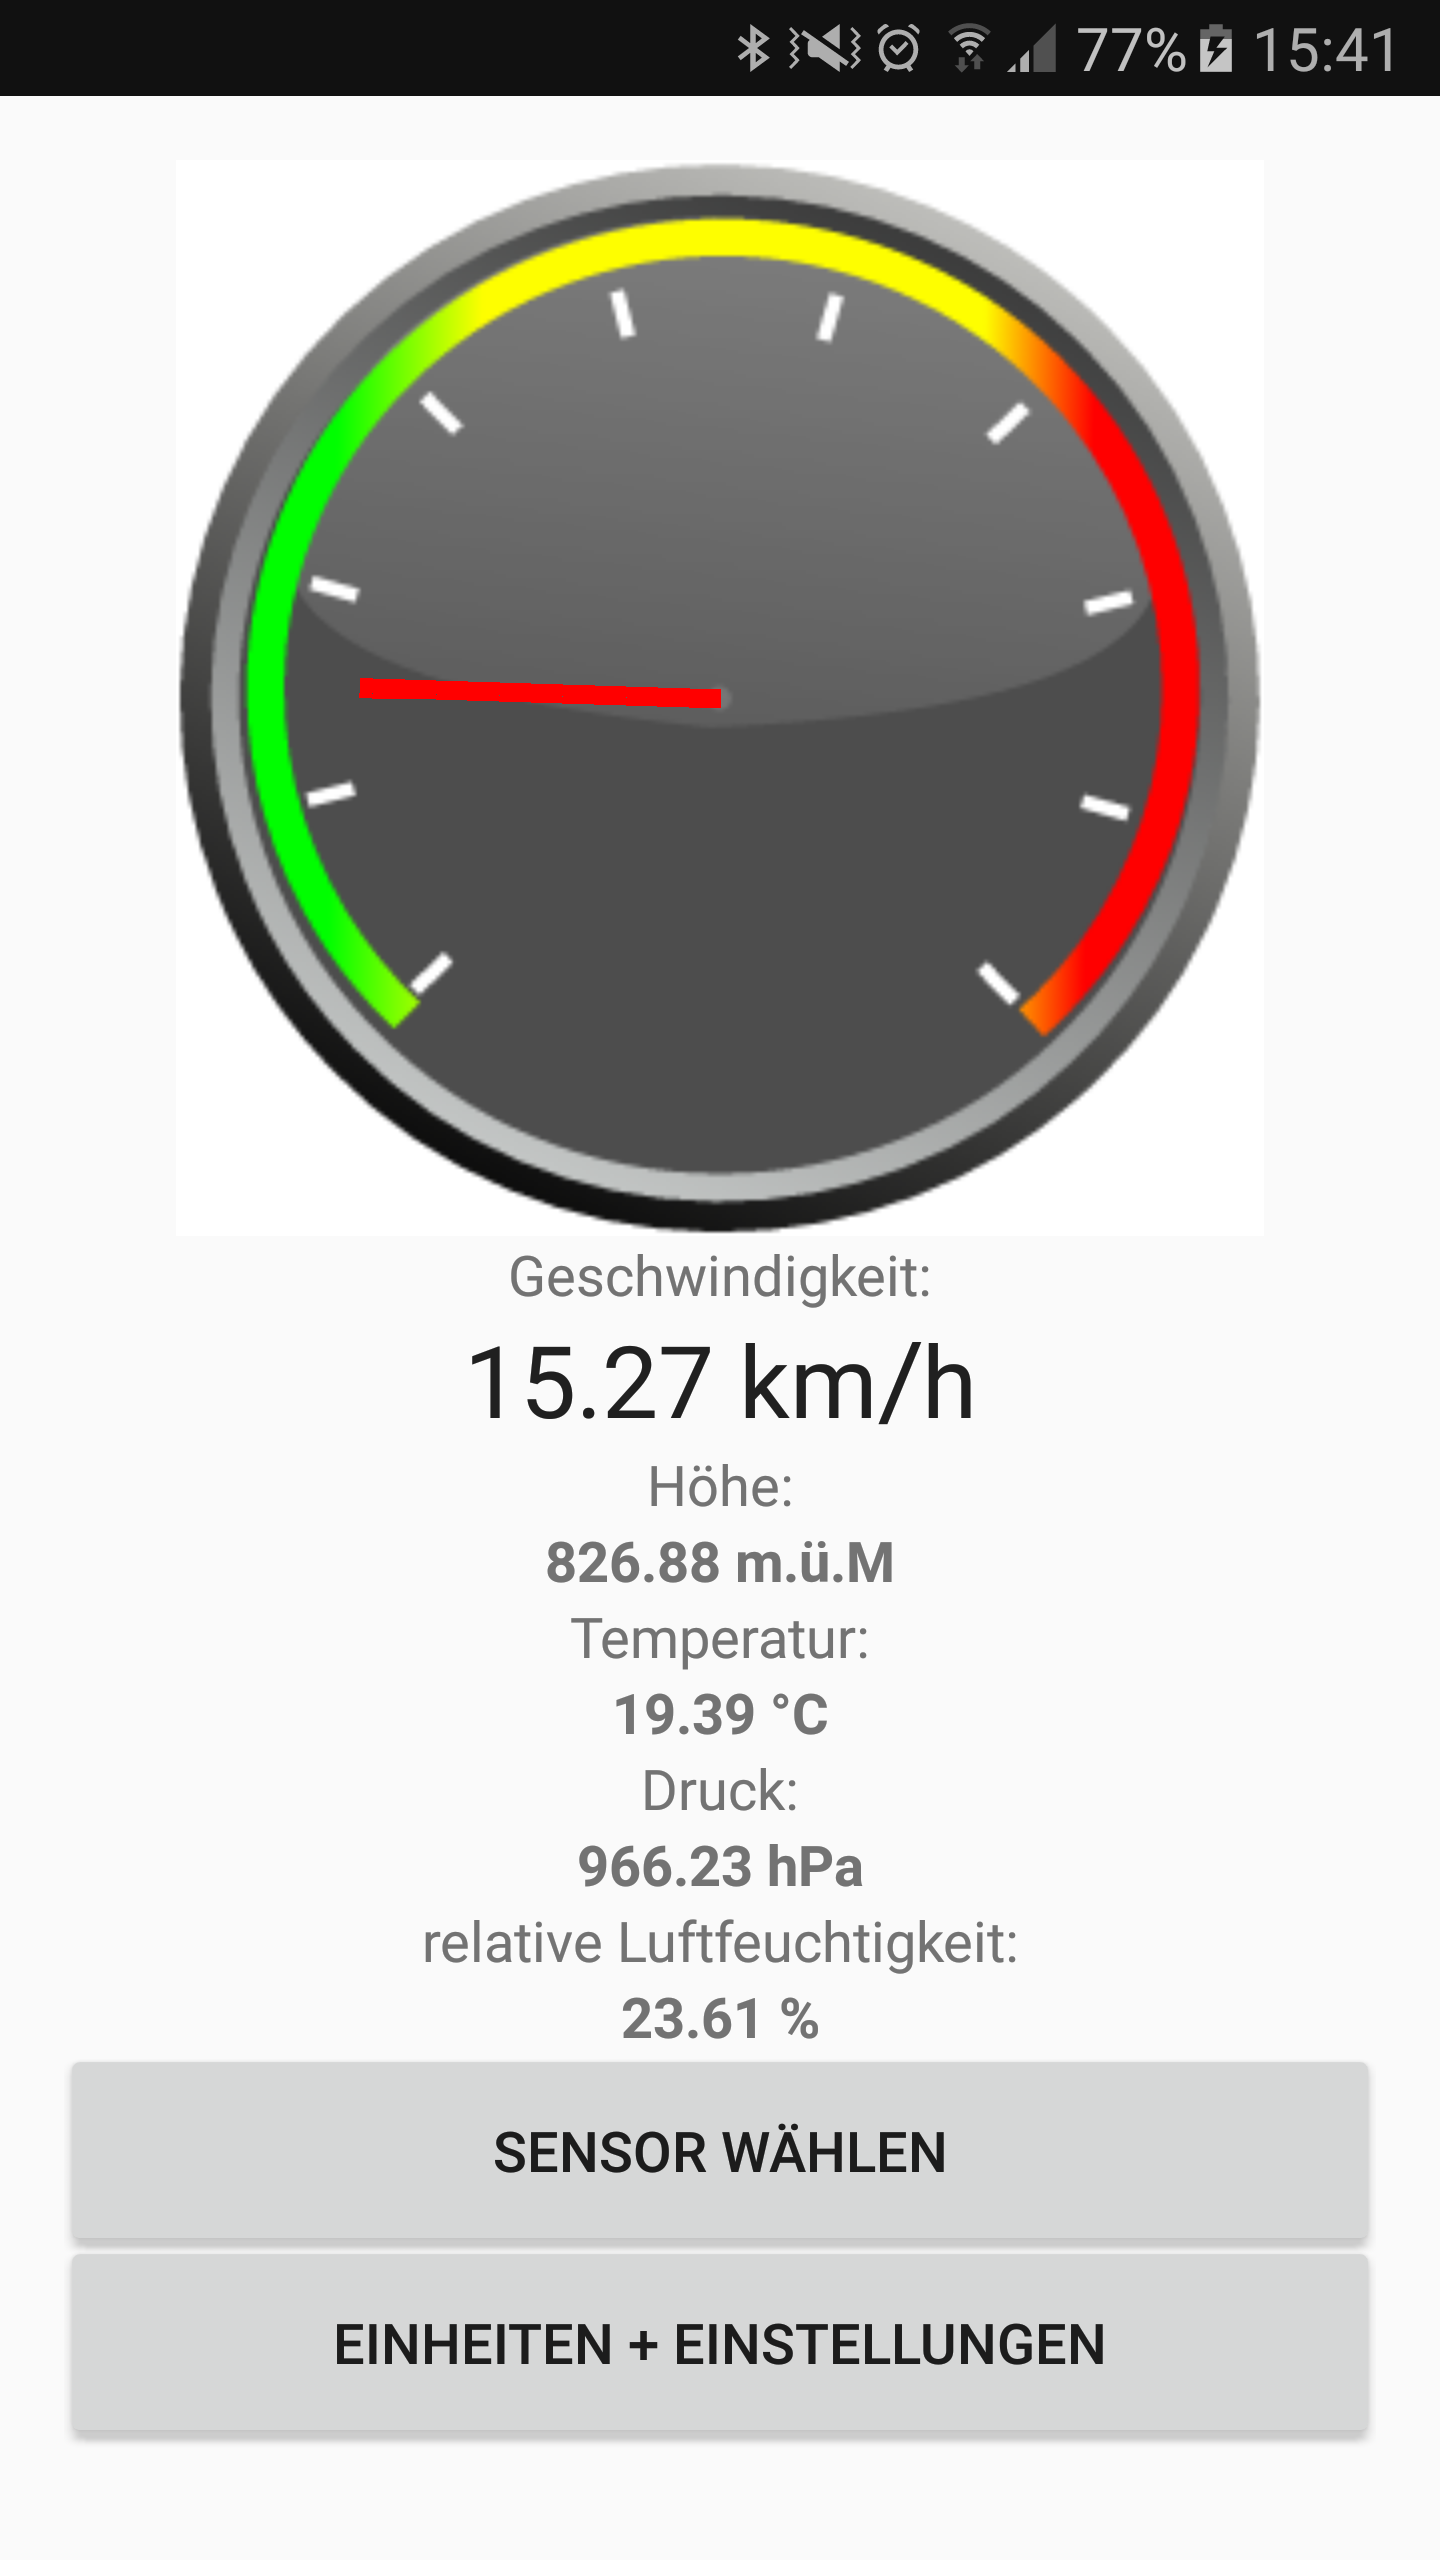
\includegraphics[width=0.5\textwidth]{4Resultate/imag/APPHomeScreen.png} 
    \caption{Startbildschirm der Applikation}
    \label{tacho}
\end{figure}

Wählt man auf dem Startbildschirm \glqq Sensor wählen\grqq, \todo{ev. besser: Sensorboard wählen} erscheint ein neuer Bildschirm. Auf diesem erscheinen nur die aktiven Bluetooth Geräte mit dem implementierten Prototypen-Filter. Der Bildschirm bildet die Sensortagadresse ab. \todo{Text: warum user das Sensor nennt. Und es dehalb so heisst und nicht Board}. Jedes Sensortag hat eine eigene Adresse und bei mehreren Prototypen im Raum, kann das entsprechende Gerät ausgewählt werden.


\begin{figure}[ht]
    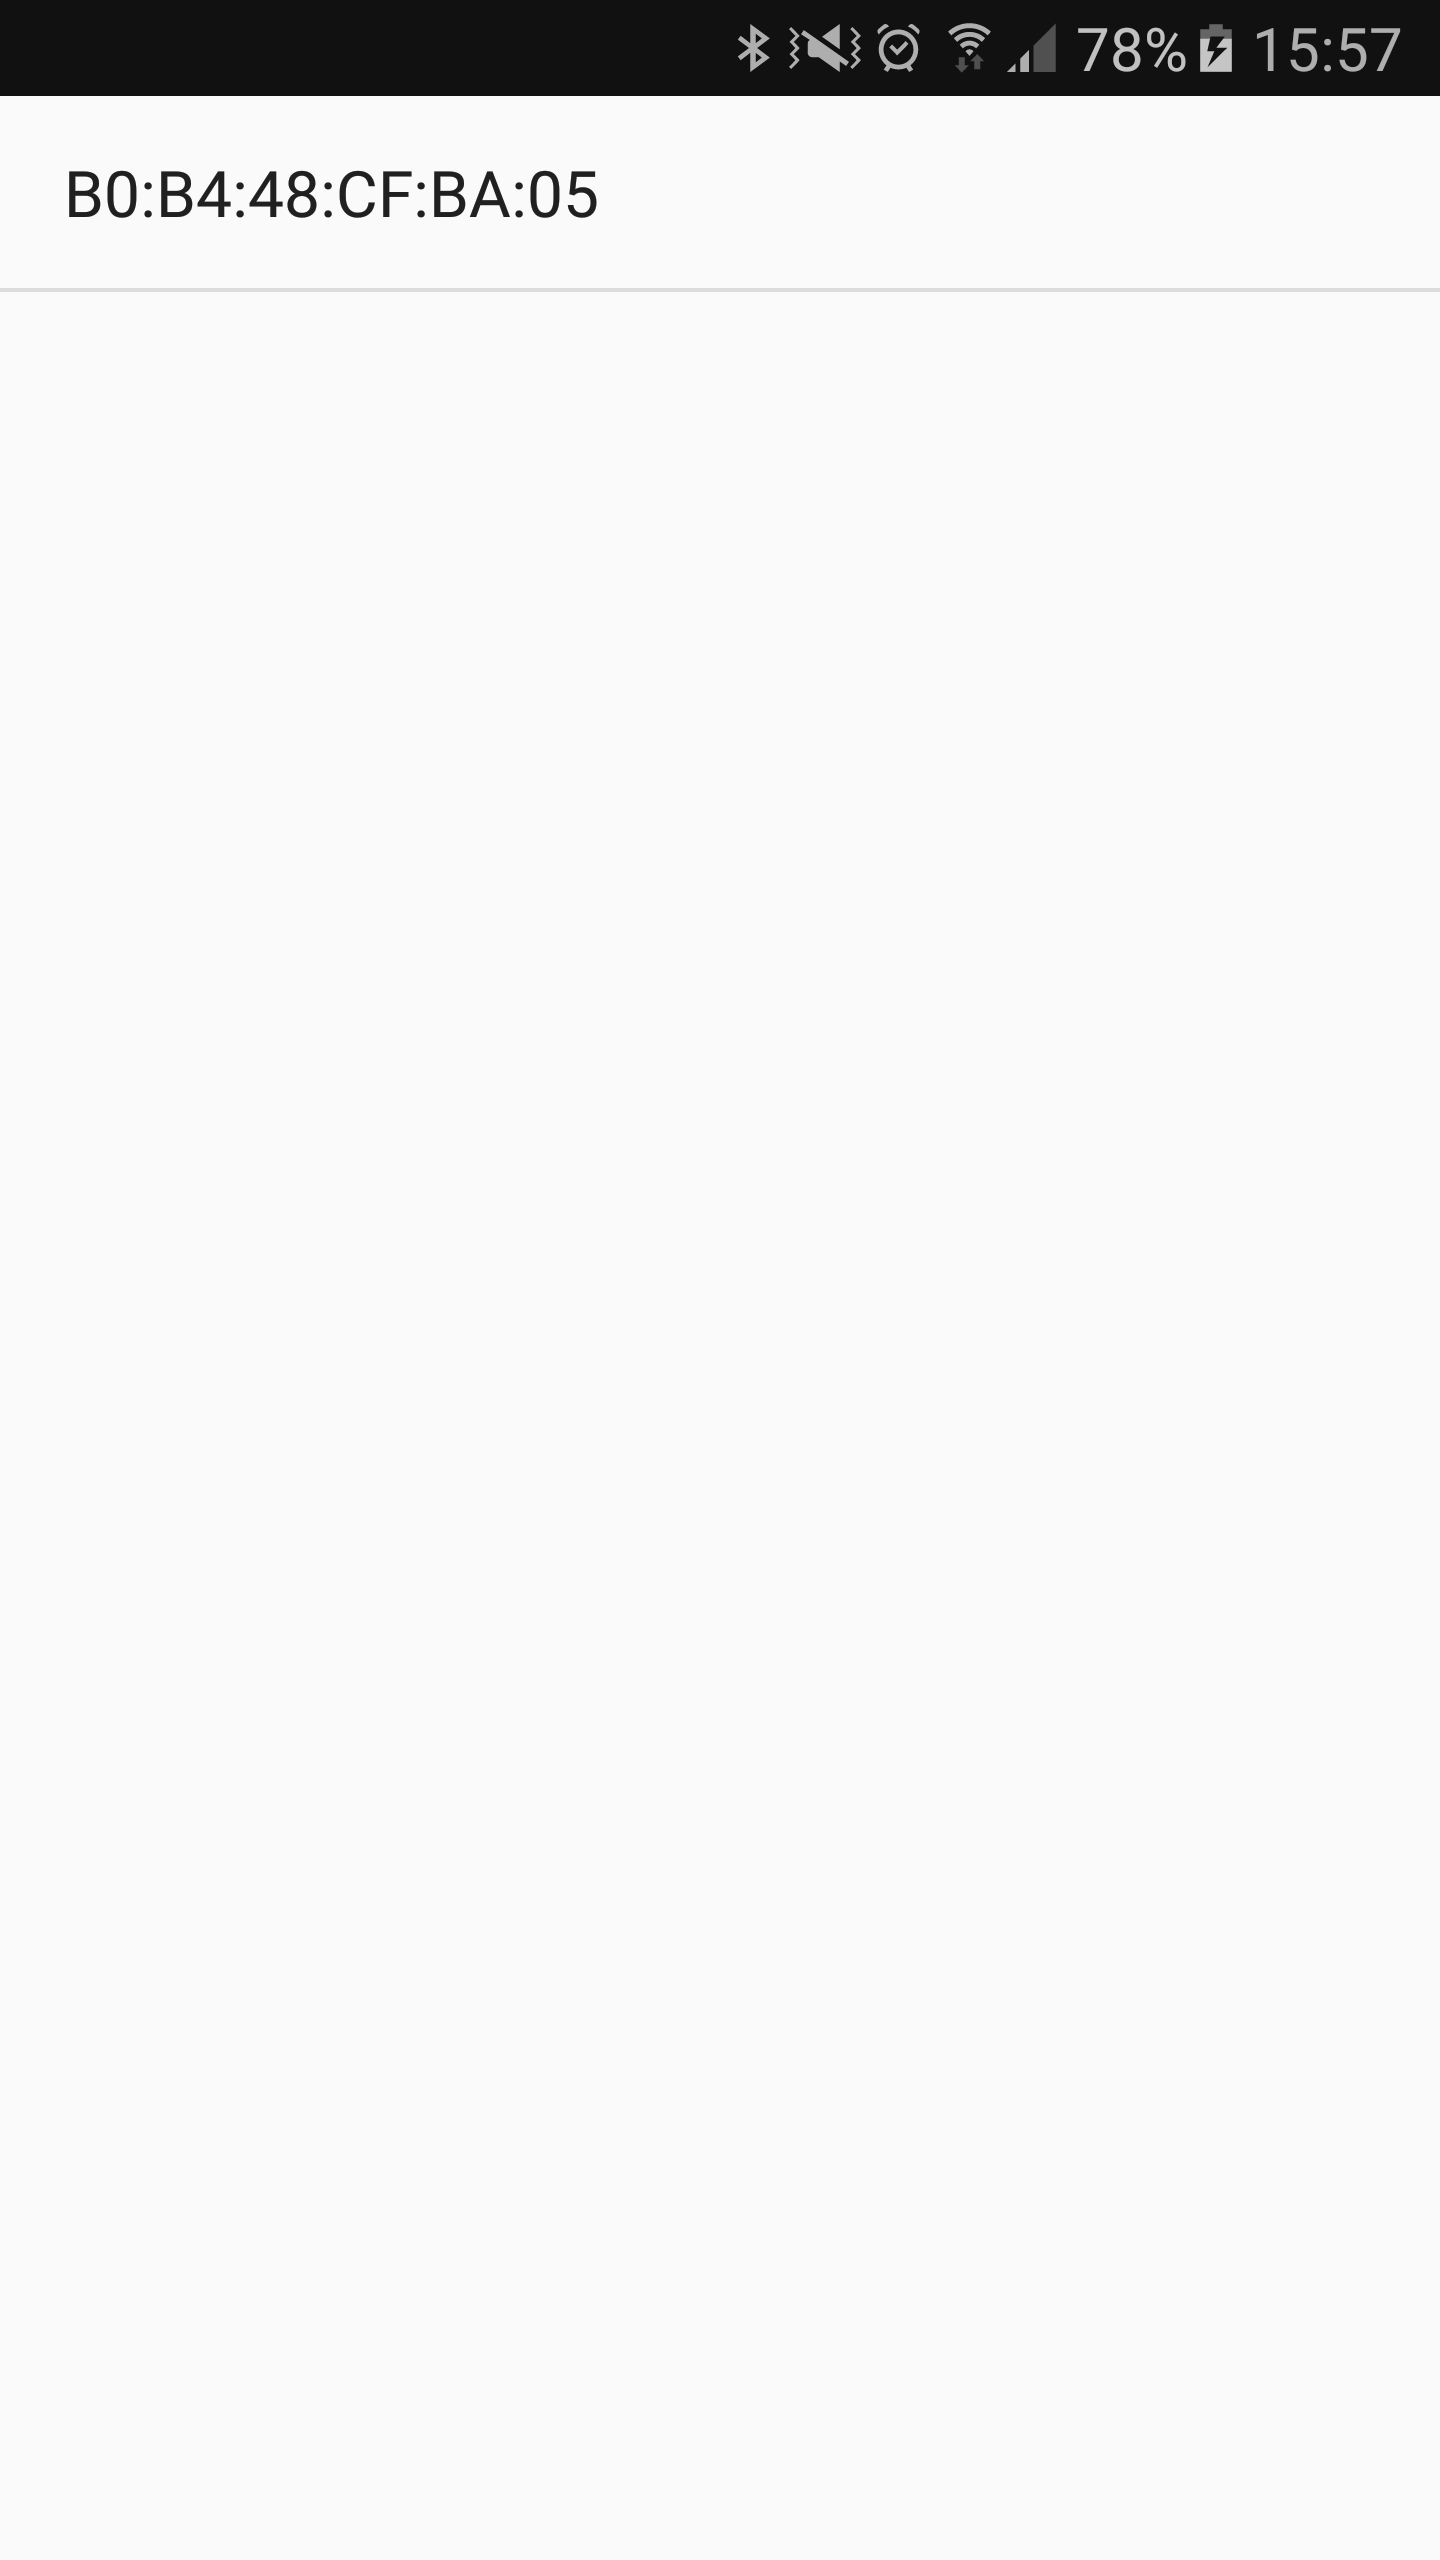
\includegraphics[width=0.5\textwidth]{4Resultate/imag/BLEAdresseAuswaehlen.png} 
    \caption{Sensortagauswahl}
    \label{sensorauswahl}
\end{figure}

Auf dem Startbildschirm befindet sich auch ein Konfigurationsknopf. In das Untermenu gelangt man, in dem man den Button "Einheiten + Einstellungen" auswählt.

\begin{figure}[ht]
    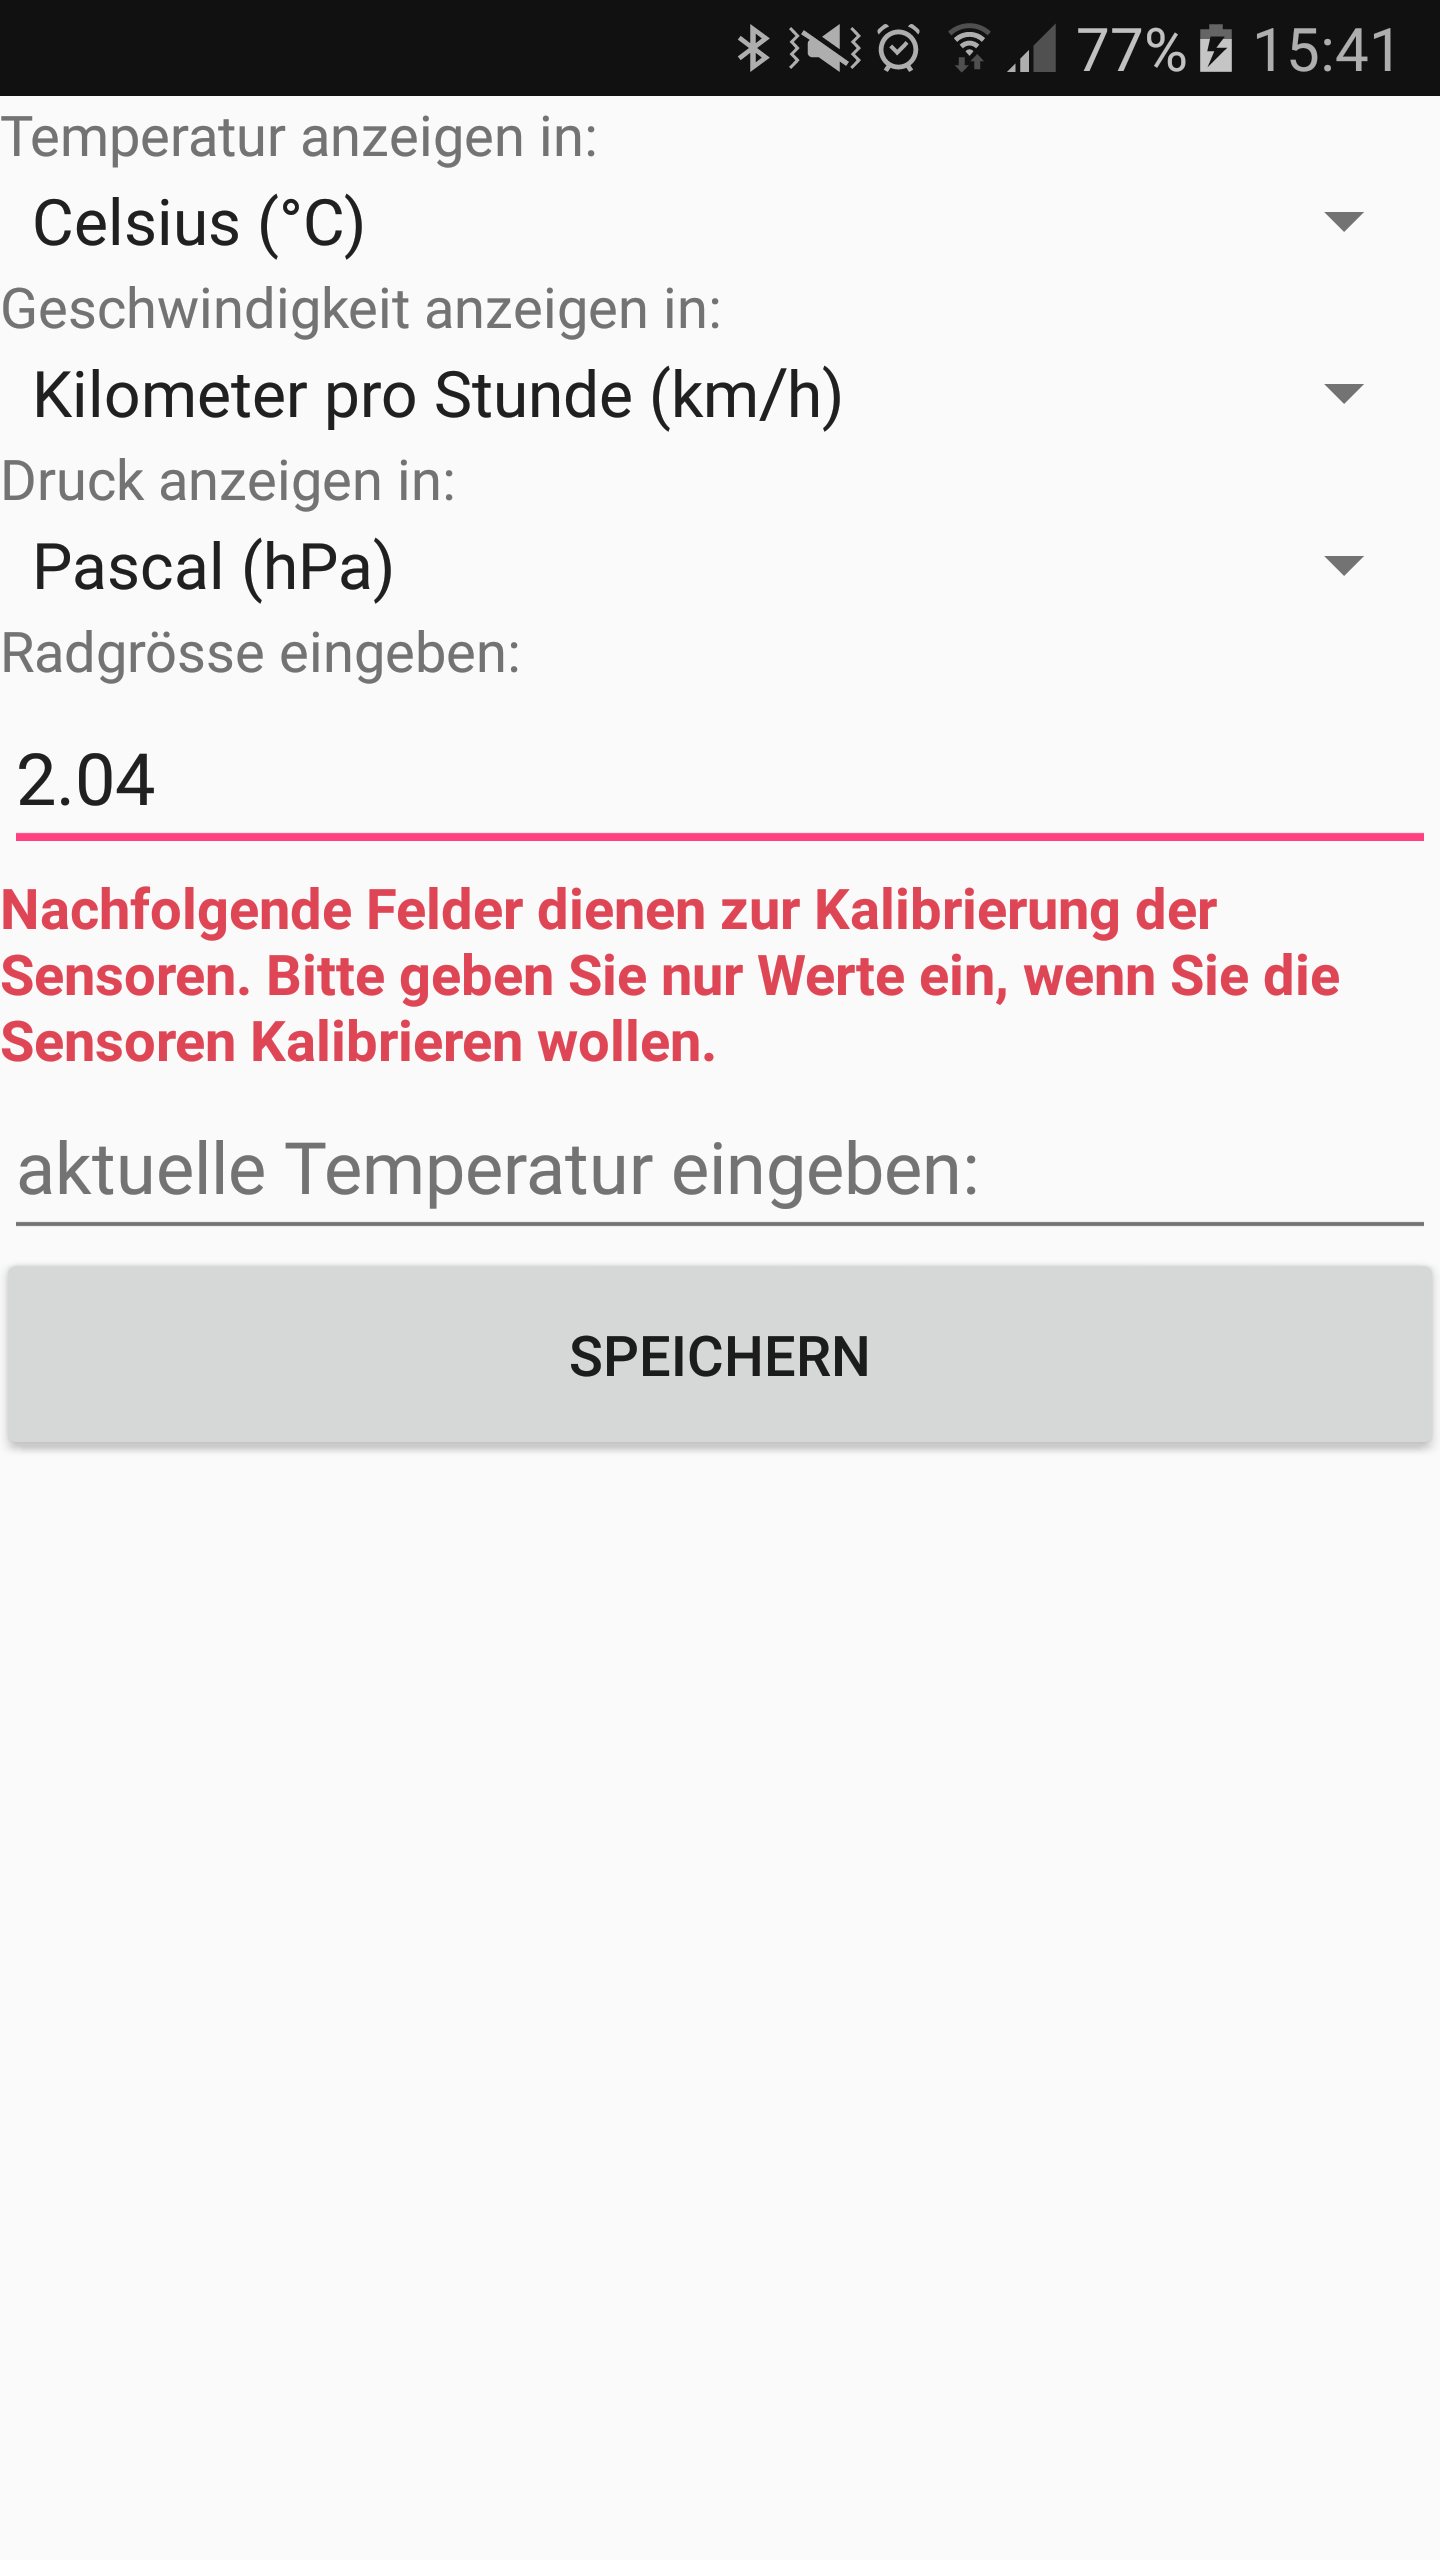
\includegraphics[width=0.5\textwidth]{4Resultate/imag/BLEEinheitenUndEinstellungenStart.png} 
    \caption{Einheiten und Einstellungen}
    \label{einheiten}
\end{figure}

Die Applikation stellt reiche Konfigurationsmöglichkeiten zur Verfügung (siehe Abbildung \ref{einheiten}. Zu jedem Sensor gehört ein Drop Down-Element, in dem die Einheiten ausgewählt werden können. Neben der Einheitenauswahl verfügt die App über die Möglichkeit, den Radumfang anzupassen und die Temperatur zu kalbrieren. 

Die Radgrösse, sprich der Radumfang, muss einstellbar sein, da die interne Geschwindigkeitsberechnung von diesem abhängt. Da die Radgrösse nicht normiert ist, konnte kein Drop Down-Element eingebaut werden. Die Zahl wird über die Tastatur in das Feld eingegeben.

Bei der Temperaturanzeige ist eine Kalibrierung eingebaut. Dies, weil alle drei Temperatursensoren auf dem Sensortag einheitlich zu hohe Werte ausgeben. Der zu hohe Temperaturwert liegt am Aufbau des Prototypen. Sensortag und Print liegen nahe aufeinander und es entsteht Wärme im Zwischenraum. Der Benutzer oder die Benutzerin kann den korrekten Wert im Kalibrationsfeld eingeben. Die nächste Temperatur, die empfangen wird, wird mit dem eingetragenen Wert verglichen und ein Offset wird eingestellt. Wird keine Kalibration eingetragen, wird die Temperatur nicht kalibriert und der Offset bleibt unverändert.

\subsubsection*{Auswählbare Einheiten}
\begin{tabbing}
    Temperatur     \quad\= Geschwindigkeit            \quad\= Druck \\[0.8ex]
    Celsius (C)    \> Kilometer pro Stunde (km/h)\> Pascal (haP)\\
    Fahrenheit (F) \> Miles per hour (mph)       \> Bar (bar)\\
    Kelvin (K)     \>                            \> Atmosph\"{a}re (atm)\\
                   \>                      \> Pound-Force per sqare inch (psi)\\
                   \>                      \> Millimeter Quecksilber (mmHG)\\
\end{tabbing} 

  
Die vorgenommenen Einstellungen werden über den Button \glqq Speichern\grqq gesichert. Danach werden die eingelesenen Sensordaten in den ausgewählten Einheiten dargestellt.

\subsection{Paketverlust}

Sensortag sendet im Advertising Mode 3 Pakete pro Sendevorgang. Gemessen wird der Paketverlust bei einer Geschwindigkeit von 20 km/h (siehe untenstehende Tabelle und \todo{Messprotokoll erwähnen}). \todo{Tabelle referenzieren}  

\subsubsection*{Paketverlust BLE-Applikation}
\begin{tabbing}
    Messperiode \quad\= Gesendete Pakete \quad\= Empfangene Pakete \quad\= Paketverlust\\[0.8ex]
    1 min  \> 38   \> 35 \> 7.9\thinspace\%  \\
    1 min  \> 37   \> 31 \> 16.2\thinspace\%  \\
    2 min  \> 75   \> 64 \> 14.7\thinspace\%  \\
    2 min  \> 77   \> 65 \> 15.6\thinspace\%  \\
    5 min  \> 193   \> 168 \> 13.0\thinspace\%  \\
    5 min  \> 190   \> 158 \> 16.8\thinspace\%  \\
    10 min  \> 345   \> 301 \> 12.8\thinspace\%  \\
    10 min  \> 349   \> 302 \> 13.5\thinspace\%  \\
\end{tabbing} 

Da der Advertising Mode keine sicher Verbindung ist, ist ein Paketverlust von rund 15\thinspace\% zu erwarten.


\subsection{Korrektheit der Daten}

Die Korrektheit der empfangenen Daten auf der Applikation wird mit einem visuellen Vergleich der Datenpakete im BLE-Sniffer von TI verglichen (siehe Abbildung \ref{sniffer}).  Die Daten im Sniffer entsprechen exakt den Daten, welche die Applikation empfängt. Der Inhalt der Daten wird somit unverfälscht übermittelt.


\todo{aktuelles Sniffer Bild} 

\begin{figure}[ht]
    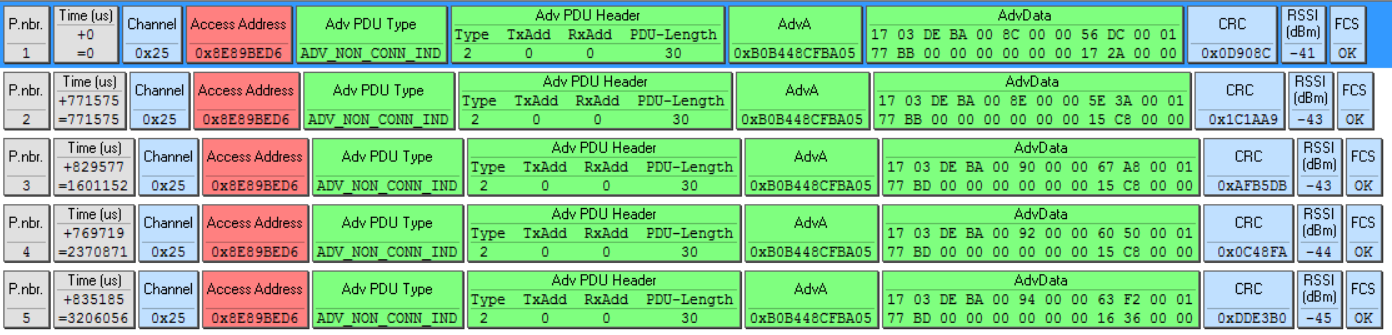
\includegraphics[width=0.5\textwidth]{4Resultate/imag/sniffer.png} 
    \caption{Snifferpaket Prototyp}
    \label{sniffer}
\end{figure}


\todo{Video zeiger (auf CD)}






